\section{Statistics Definitions}

These terms come up all the time throughout statistics, so it is important to know what these mean as you go into studying for this course.

\subsection{Descriptive VS Inferential Statistics}

\begin{itemize}
    \item \bf{Descriptive statistics} deals simply with the data presented and the story being told by that data. We simply care about being able to analyze data.
    \item \bf{Inferential statistics} deals with using the data presented to make arguments/statements about various issues in populations
\end{itemize}

Statistics classes like this one are all about learning BOTH skills, starting with learning descriptive statistics and then moving on to learning inferential statistics.



\subsection{Parameters VS Statistics}

\begin{itemize}
    \item \bf{Statistics:} values that describe a sample
    \item \bf{Parameters:} values that describe a population/population model
\end{itemize}

The goal of inferential statistics is to use statistics to infer on the true values of parameters. \it{EXAMPLE: Computing the mean GPA of 35 students from a high school is a statistic. We can use this average to make inferences on the mean GPA of all of the students in the high school, a parameter.}


\subsection{Quantitative VS Categorical Data}

\begin{itemize}
    \item \bf{Quantitative data:} the specifics of data, data that can answer "how much" or "how many" questions
    \begin{itemize}
        \item EXAMPLES: heights, speeds, weights, calories burnt, scores on exams, etc.
    \end{itemize}

    \item \bf{Categorical data:} data that can be sorted based on a non-quantitative characteristic
    \begin{itemize}
        \item EXAMPLES: gender, political party preference, eye color, level of education, etc.
    \end{itemize}
\end{itemize}

Sometimes, it can be hard to distinguish if a piece of data is quantitative or categorical (for example, grade of a student can be thought of as putting students into categories but it also is a way of quantitatively measuring the number of years of education a student has completed). If that is the case, paying attention to the context of where the data is presented to determine if the data is categorical or quantitative.



\subsection{Discrete and Continuous Variables}

These are ways to describe quantitative variables.

\begin{itemize}
    \item \bf{Discrete variables:} variables that can only take on specific types of values (such as whole numbers)
    \item \bf{Continuous variables:} variables that can be measured over an interval 
\end{itemize}

Generally in the scope of this class, this distinction is important because our data is always discrete while the statistical models that we build are generally continuous.




\section{Graphical Analysis}

Graphs are an important part of statistics, and being able to analyze graphs is a crucial skill. To be able to analyze a graph well, the following three elements must ALWAYS be touched on in any analysis of data:

\begin{itemize}
    \item \bf{SHAPE}
    \item \bf{CENTER}
    \item \bf{SPREAD}
    \item \bf{OUTLIERS}
    \item \bf{GAPS/CLUSTERS}
\end{itemize}



\subsection{Shape}

When talking about statistics, it is important to notice what the shape of the graph is. The different types of shapes are explained below:

\begin{itemize}
    \item \bf{symmetric:} the data has some symmetry about some axis)
    \item \bf{bell-shaped:} the graph looks like the shape of the bell (like a Normal distribution)
    \item \bf{skewed left:} the tail of the data is on the left
    \item \bf{skewed right:} the tail of the data is on the right
    \item \bf{bimodal:} multiple points which have multiple data values
    \item \bf{uniform:} frequencies of values are more/less constant
\end{itemize}


\subsection{Center}

To describe the center, of a distribution, you can use either the \it{median} or the \it{mean}, and there are reasons for using either one.

\begin{itemize}
    \item \bf{mean:} The sum of all the data points divided by the total number of data points. The formula is as follows: $\bar{x} = \frac{\sum{x}}{n}$ where $x$ is the actual value of the specific data point and $n$ is the total number of data points. The $\sum$ symbol means "add up all the values of $x$." 
    \begin{itemize}
        \item When talking about the mean in the context of a sample (aka a \it{statistic}) use the symbol $\bar{x}$ for the mean
        \item When talking about the mean in the context of a population (aka a \it{parameter}), use the symbol $\mu$
        \item The mean is NOT a \bf{resistant statistic}, which means that the mean could change a lot depending on what values are added to the dataset
    \end{itemize}

    \item \bf{median:} the value that cuts the entire data set in half. This means that 50\% of the dataset are greater than the mean and 50\% of the dataset are less than the mean. The mean is always at the $\frac{n+1}/2$ position in the dataset if the data is sorted in numerical order.
    \begin{itemize}
        \item If there are an odd number of data points in the data set, then there is one value in the middle
        \item If there are an even number of data points in the data set, then the mean of the middle two values are the median
        \item The median is a \bf{resistant statistic}, which means that the value of the median will not drastically change no matter what values are added to the dataset.
    \end{itemize}
\end{itemize}

\begin{definition}[How to Choose Your Center]{def1:label}
    If the shape of the data is \it{symmetric} and/or \it{centered}, then use the \bf{mean} when talking about center. If the data is \it{skewed} in any way, use the \bf{median} when talking about center.
\end{definition}


\subsection{Spread}

There are two different statistics that we can use to describe the spread (or how far about all the data points are) in a dataset:

\begin{itemize}
    \item \bf{standard deviation:} This value measures the average distance any data point in the dataset is away from the mean
    \begin{itemize}
        \item Formula: $s_x = \sqrt{\frac{\sum (x_i - \bar{x})^2}{n-1}}$
        \item If you are talking about the standard deviation of a population (in other words a \it{statistic}), you should use the symbol $s_x$
        \item If you are talking about the standard deviation of a population (in other words a \it{parameter}), you should use the symbol $\sigma$
        \item the standard deviation is NOT a \bf{resistant statistic}, so adding new values to the dataset could drastically impact the standard deviation
    \end{itemize}

    \item \bf{interquartile range (IQR):} this value measures the difference between the third quartile (Q3) and the first quartile (Q1)
    \begin{itemize}
        \item Formula: Q3 - Q1
        \item Q1: the median of all the values that are less than the median (25\% mark)
        \item Q3: the median of all the values that are greater than the median (75\% mark)
        \item the IQR is a \bf{resistant statistic} so adding new values to the dataset will not drastically change the value of the IQR
    \end{itemize}
\end{itemize}

\begin{definition}[Choosing Your Spread]{def2:label}
    If you used the \it{mean} to talk about your center, then you must use the \bf{standard deviation} to talk about the spread. If you use the \it{median} to talk about your cennter, then you must use the \bf{interquartile range} to talk about the spread.
\end{definition}


\subsection{Outliers}

An \bf{outlier} is a data point that is significantly separated from every other point in the data set. It is important to talk about outliers when analyzing data, and there is an algorithm to help you determine what data points are considered outliers.

\begin{definition}[The Outlier Algorithm]{def3:label}
    To find potential outlier(s) in your dataset, follow these steps:

    \begin{enumerate}
        \item Calculate the IQR
        \item Multiply the IQR by 1.5
        \item Compute $Q1 - 1.5 \cdot IQR$ and $Q3 + 1.5 \cdot IQR$
        \item Any data point that is below $Q1 - 1.5 \cdot IQR$ is an outlier
        \item Any data point that is above $Q3 + 1.5 \cdot IQR$ is an outlier
    \end{enumerate}
\end{definition}

Outliers contain valuable information since outliers can reveal something unusual/unexpected about a given dataset that is important for a statistician to know about. An outlier could potentially reveal a problem/inconsistency without how the data was generated. \newpage


\subsection{The Five Number Summary}

The \bf{five number summary} of a dataset contains the values of 5 different statistics that can help you when analyzing one-variable data. It contains these 5 statistics:

\begin{itemize}
    \item MIN VALUE  
    \item Q1
    \item MEDIAN 
    \item Q3
    \item MAX VALUE
\end{itemize}

If you give your calculator a list of data, your calculator can compute a five number summary for you, as well as tell you the median and standard deviation. You can also use a box and whisker plot to model the 5 number summary. In a box and whisker plot, the edges of the box are the Q1 and Q3 labels, and the line splitting the box is the median. This lets you find the values in the 5 number summary fairly easily. Outliers are also marked separately with their own points. 



\section{Z-Scores and Normal Distributions}

\subsection{z-scores}

We can denote the position of a data point in a dataset by describing how many standard deviations the data point is away from the mean. The statistic that can tell us this is the \bf{z-score}.

\begin{definition}[The Z-Score]{def3:label}
    The formula for the z-score of a certain value is as follows:

    $$
    z_{xi} = \frac{x_i - \bar{x}}{s_x}
    $$

    For example, the value $z_2 = 1.5$ tells us that the value 2 is 1.5 standard deviations above the mean. Likewise, the value $z_-1 = -2$ tells us that the value -1 is 2 standard deviations below the mean.\\

    If you calculate the z-scores of every item in a distribution, then the distribution of z-scores will always have a mean of 0 and a standard deviation of 1.
\end{definition}



\subsection{Normal Distribution}

A \bf{Normal curve} is a graph that looks bell-shaped and symmetric. It is used to generalize the behavior of data when the data has lots and lots of values associated with it. A Normal curve looks something like this: \newpage

\begin{center}
    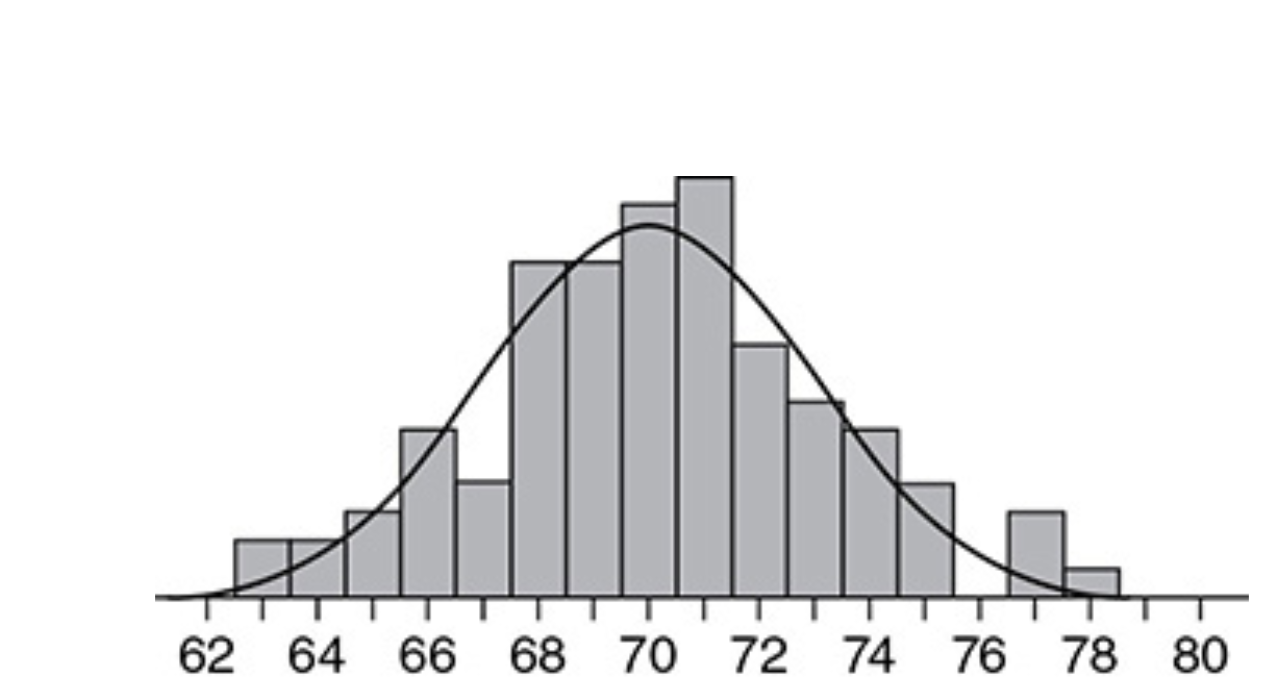
\includegraphics[width=\textwidth]{chapters/unit1/images/fig1.1.PNG}
\end{center}

The black curve on top of the graph is the Normal curve. The area under the entire normal curve has an area of 1.


\begin{definition}[The 68-95-99.7 Rule]{def4:label}
    \it{APPROXIMATELY} 68\% of the data points in a Normal distribution are within 1 standard deviation of the mean.\\

    \it{APPROXIMATELY} 95\% of the data points in a Normal distribution are within 2 standard deviation of the mean.\\

    \it{APPROXIMATELY} 99.7\% of the data points in a Normal distribution are within 3 standard deviation of the mean.\\
\end{definition}


\subsection{Standard Normal Distributions}

A standard Normal distribution is a theoretical distribution, so that means that we will need to use $\mu$ and $\sigma$. Suppose we have some variable $X$ which has a Normal distribution with a mean of $\mu$ and a standard deviation of $\sigma$. First of all, we can denote this Normal distribution using the notation "$X$ has $N(\mu, \sigma)$". However, every Normal distribution also has a related distribution that we can find by \bf{standardizing} the data in the distribution. Doing this produces the \bf{standard Normal distribution}. To begin this process, you first need to convert all of the data into z-scores using the following formula:

$$
    z = \frac{x-\mu}{\sigma}
$$

By doing this, the distribution of z-scores will have a mean of 0 and a standard deviation of 1. This would also mean that the distribution of z-scores is Normal, so z has $N(0,1)$. Then by following the 68-95-99.7 rule, we then know that 68\% of all data points lie between $z=-1$ and $z=1$ and that 95\% of the data points lie between $z=-2$ and $z=2$ and that 99.7\% of the data are between $z=-3$ and $z=3$. \\

Since a lot of data distributions that exist in the world can be approximated with a Normal distribution, then it is possible to compute the standard Normal distribution by using either a calculator or Table A (found in the Appendix chapter at the end of this document).\\

\bf{NOTE:} If you choose to use you calculator to compute the area under the Normal curve, then use the normalcdf function. The syntax for the function is normalcdf(upper bound, lower bound, mean, standard deviation). however, if you know you are working with a standard Normal distribution, then you can just put in the upper and lower bounds because the calculator will automatically add the mean and standard deviation.